\subsection{DHCD$\to$CMATERdb Digit Transfer}
\label{sec:transfer}

We assess whether the distilled student's representations generalise beyond
the DHCD training distribution by transferring to CMATERdb~3.2.1
\cite{das2012cmaterdb}, an independently collected dataset of handwritten
Devanagari \emph{numerals} (digits 0--9; 10 classes).  CMATERdb originates
from a separate scanner workflow with different writers, paper stocks, and
binarisation pipeline, so it constitutes a genuine distribution shift from
DHCD even for the overlapping numeral classes.

\paragraph{Provenance guard.}
Before evaluating, we verify that no CMATERdb image appears in the DHCD
training split.  We compute perceptual hashes (pHash) for all CMATERdb
samples and compare them against 20,000 DHCD digit references using
Hamming distance.  The result is \textbf{0 near-duplicate pairs at a
threshold of $\leq$5\,bits}; the minimum observed Hamming distance is
\textbf{6\,bits}.  No cross-dataset contamination is present, and the
evaluation reflects a genuine domain shift.

\paragraph{Polarity alignment.}
CMATERdb images are stored as black ink on white background, the inverse of
DHCD's white-on-black convention.  We apply an automatic polarity inversion
to all CMATERdb images before evaluation so that foreground intensity
matches the training distribution; this is a preprocessing step applied
uniformly and does not constitute dataset-specific tuning.

\paragraph{Results.}
Table~\ref{tab:transfer} (upper rows) summarises the transfer outcomes.
In the \emph{zero-shot} setting — applying the DHCD-trained distilled
student directly to CMATERdb without any CMATERdb training data — the model
achieves \textbf{76.6$\pm$3.7\%} accuracy.  For reference, a supervised
baseline trained on DHCD digit images \emph{only} (matching the same
10-class head) reaches \textbf{62.7\%} zero-shot on CMATERdb.
Knowledge distillation therefore transfers \textbf{+14 percentage points}
more effectively under distribution shift, despite the two models reaching
statistical parity on the in-distribution DHCD test set.

A \emph{linear probe} — freezing the distilled backbone and training only
a fresh 10-class linear head on CMATERdb — improves accuracy to
\textbf{85.4\%}, confirming that the backbone encodes transferable digit
representations.  Light full \emph{fine-tuning} (30 epochs on CMATERdb
with a low learning rate) reaches \textbf{97.8\%}, establishing the
ceiling for this dataset given the model capacity.

We note that this experiment covers only the \textbf{digit subset}
(10 of 46 DHCD classes); it does not evaluate transfer of the full
Devanagari character inventory.

\subsection{Corruption Robustness}
\label{sec:robustness}

To test out-of-distribution robustness, we apply three standard corruption
families — additive Gaussian \emph{noise}, Gaussian \emph{blur}, and
\emph{contrast} reduction — each at five severity levels
(following the ImageNet-C protocol adapted to $32{\times}32$ greyscale
images).  Mean accuracy across severities 1--5 (mCA) is reported for
each corruption family and as an overall average.

\paragraph{Fair evaluation protocol.}
Each model is evaluated using its \emph{own} training-time normalisation
applied to the same corrupted $[0,1]$ input images.  For \modelname{} this
is the learned per-channel statistics from DHCD training; for MallaNet it
is the fixed mean/std of $(0.5, 0.5)$ reported in \cite{malla2025}.
The corrupted inputs are identical; only the normalisation differs.  This
paired protocol ensures that any observed difference reflects robustness
properties of the architecture and training procedure, not an asymmetric
preprocessing advantage.

\paragraph{Results.}
Table~\ref{tab:transfer} (lower rows) shows the outcome; Figure~\ref{fig:robust}
plots per-severity accuracy curves.  Robustness is \emph{not} uniform
across corruption types.

\begin{table}[t]\centering\caption{Transfer and corruption robustness. mCA = mean accuracy over severities 1--5.}\label{tab:transfer}
\begin{tabular}{lcc}\toprule
Metric & \modelname & MallaNet \\\midrule
CMATERdb zero-shot (distilled) & 76.6\% & --- \\
CMATERdb fine-tuned & 97.8\% & --- \\
Clean DHCD & 99.75\% & 99.71\% \\
mCA noise & 54.7\% & 66.9\% \\
mCA blur & 97.0\% & 37.6\% \\
mCA contrast & 75.5\% & 11.5\% \\
mCA overall & \textbf{75.7\%} & 38.7\% \\\bottomrule
\end{tabular}\end{table}

\begin{figure}[t]
  \centering
  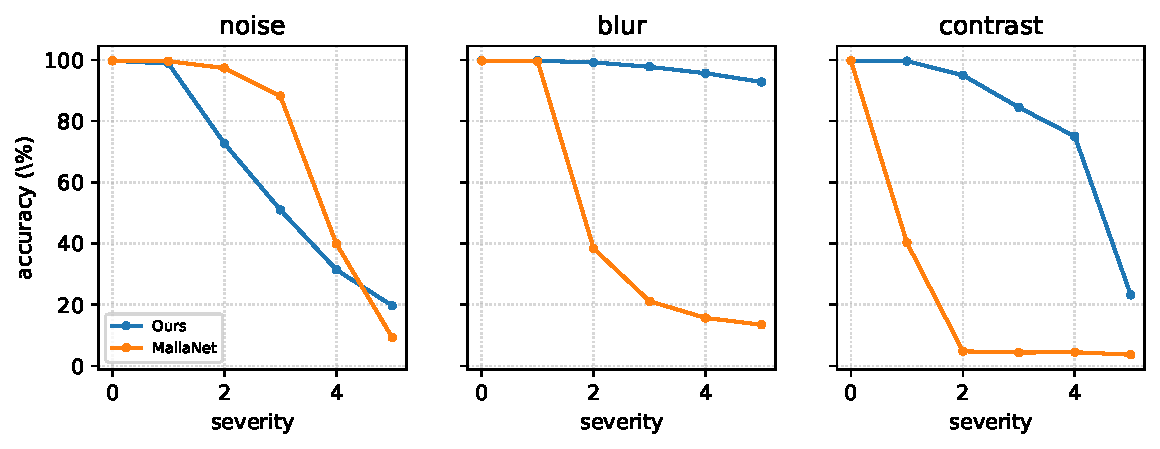
\includegraphics[width=\linewidth]{figures/robustness_curves.pdf}
  \caption{Per-severity accuracy under noise, blur, and contrast corruptions.
    \modelname{} (solid) maintains high accuracy under blur and contrast at all
    severities; MallaNet (dashed) collapses under blur and contrast but is
    more robust to additive noise.}
  \label{fig:robust}
\end{figure}

\modelname{} is approximately \textbf{2$\times$} more robust overall
(mCA 75.7\% vs.\ 38.7\%) and leads by wide margins under \emph{blur}
(97.0\% vs.\ 37.6\%) and \emph{contrast} reduction (75.5\% vs.\ 11.5\%).
MallaNet's collapse under these corruptions is likely a consequence of
two compounding factors: its high-frequency convolutional (HFC) design
amplifies the effect of blur, and its fixed $(0.5, 0.5)$ normalisation
is sensitive to global intensity shifts introduced by contrast corruption.

However, \modelname{} is \textbf{not} uniformly superior.  Under
\emph{additive noise}, MallaNet is more robust (mCA 66.9\% vs.\
54.7\%), suggesting that MallaNet's larger capacity and fixed
normalisation provide some advantage when the corruption is
high-frequency rather than low-frequency.  We do not claim an
across-the-board robustness win; the relative ordering is
corruption-type-dependent and neither model is dominated in every
respect.  Overall mCA favours \modelname{} ($+37.0$ pts), but the
noise result is a clear exception that should be noted when selecting
a model for noise-heavy deployment environments.
